\documentclass[conference]{IEEEtran}
\IEEEoverridecommandlockouts
\usepackage{cite}
\usepackage{amsmath,amssymb}
\usepackage{graphicx}
\usepackage{booktabs}
\usepackage{tikz}
\usetikzlibrary{positioning,arrows.meta,fit,backgrounds}
\usepackage{url}
\usepackage[hidelinks]{hyperref}
\graphicspath{{../screenshots/}}

\begin{document}

\title{PHYSIOS: A Standalone Operating Environment for\\
Imitation-Learning Workflows on Low-Cost Robot Arms}

\author{\IEEEauthorblockN{[Author names]}
\IEEEauthorblockA{[Department, Institution]\\{}
[City, Country]\\{}
Technical report, PHYSIOS 1.1.0, 11 November 2026}}

\maketitle

\begin{abstract}
Learning manipulation skills from human demonstrations has become practical on inexpensive
hardware, but the surrounding workflow---planning demonstrations, recording them, curating the
data, training and diagnosing a policy, and running it on the robot under supervision---is
usually spread across scripts, notebooks and loosely coupled web tools. This paper describes
PHYSIOS, an independent application that unifies this workflow for the SO-101 arm on top of the
ROBOTIS Physical AI Tools stack, ROS~2 and LeRobot. PHYSIOS adds a standard-library gateway
that fronts the existing robot-side node, a host training service and camera server through
one versioned API, and a dependency-light web frontend organised as a numbered workflow.
Design goals were independence from the earlier user interface, unchanged robot-side code,
explicit operator initiation for every motion, and honest reporting of unavailable services.
We describe the architecture, the safety model (typed confirmations, server-enforced motion
gating, a joint envelope derived from the demonstrations, heartbeat-based holding, and a staged
readiness process for custom robots), the training-optimisation loop based on controlled trials
from a pre-problem checkpoint, and a compact interface design. Validation so far uses
real back-end code with simulated robot and trainer stand-ins: 20 gateway tests, 8 frontend
tests, 91 training-service tests, 45 planning tests, a 14-step browser walk-through, a
sign-in walk-through and a containerised deployment. Verification on the physical robot and
with GPU training is outstanding and is listed explicitly.
\end{abstract}

\begin{IEEEkeywords}
imitation learning, robot learning infrastructure, vision-language-action models, ROS~2,
LeRobot, human--robot interaction, safety, web-based robot interfaces
\end{IEEEkeywords}

\section{Introduction}
Vision-language-action (VLA) models such as RT-2~\cite{rt2}, OpenVLA~\cite{openvla},
$\pi_0$~\cite{pi0} and the compact SmolVLA~\cite{smolvla}, together with action-chunking and
diffusion policies~\cite{act,diffusion}, have made it realistic to teach a low-cost arm a
task from a few dozen teleoperated demonstrations. Open libraries such as
LeRobot~\cite{lerobot} provide data formats, training scripts and policies; ROS~2~\cite{ros2}
provides the robot middleware.

What remains difficult for a small lab is the \emph{workflow}. In the project that motivated
this work, an operator recorded 39 leader--follower demonstrations of a cube pick-and-place
task with two cameras and fine-tuned SmolVLA on them. Offline, the policy reproduced the
demonstrations closely and on the robot it reached the cube; a reliable grasp required better
matched camera conditions and more data. Each of these steps lived in a different tool: a
ROS-based recording interface, command-line training, ad hoc evaluation and separate rollout
scripts. Decisions such as \emph{which} demonstrations to collect next or \emph{whether} a
training run diverged were made by inspecting logs by hand.

PHYSIOS (``The Operating System for Physical Intelligence'') addresses this by providing one
independent application for the complete loop: plan $\rightarrow$ record $\rightarrow$ curate
$\rightarrow$ train and optimise $\rightarrow$ evaluate $\rightarrow$ run under supervision. Its
contributions are:
\begin{itemize}
\item an architecture that adds an application layer \emph{without modifying} the robot-side
node, so an existing SO-101 setup keeps working unchanged (Section~\ref{sec:arch});
\item a safety model in which every motion requires explicit operator initiation and is gated by
the server, not only by the user interface (Section~\ref{sec:safety});
\item a training-optimisation procedure based on controlled trials from the last healthy
checkpoint (Section~\ref{sec:workflow});
\item an interface design that favours density and status visibility for operators
(Section~\ref{sec:ui}); and
\item a transparent validation report that separates simulated from physical evidence
(Section~\ref{sec:validation}).
\end{itemize}

\section{Background}
\textbf{ROBOTIS Physical AI Tools}~\cite{pat} combine LeRobot with a ROS~2 node
(\texttt{physical\_ai\_server}) that records LeRobot datasets from camera and joint topics, runs
on-robot inference and exposes ROS services such as \texttt{/task/command} and
\texttt{/set\_robot\_type}. The ROS~2 graph uses the Zenoh middleware~\cite{zenoh}; browsers
reach it through rosbridge~\cite{rosbridge}, which maps ROS services and topics to JSON over
WebSockets~\cite{rfc6455}. Earlier versions of our work (v2--v4) extended this stack with a
planning engine for demonstration collection, a host training service (\texttt{pam\_trainer})
that drives \texttt{lerobot-train} in the operator's Python environment, an optimisation
controller and a custom-robot library with URDF validation. These capabilities were reachable
only through the original web interface. PHYSIOS keeps the back ends and replaces the
application layer.

\section{Requirements}
The design was driven by six requirements:
\begin{enumerate}
\item[R1] \emph{Independence.} Own frontend, API, navigation, configuration, start-up and
shut-down; no dependency on the earlier interface at run time.
\item[R2] \emph{Reuse without modification.} The robot-side node, its ROS interfaces, the dataset
format and storage locations stay unchanged.
\item[R3] \emph{Explicit motion.} No start-up path may move the robot; every motion needs a
deliberate operator action, enforced server-side.
\item[R4] \emph{Truthful state.} Unavailable services are reported with their cause and a
remedy; no placeholder data.
\item[R5] \emph{Operator efficiency.} Dense, consistent screens that show robot, data and
training state at a glance, on desktop and small screens.
\item[R6] \emph{Deployability.} Script-based and containerised installation on the robot PC,
optional authentication for network access.
\end{enumerate}

\section{Architecture}\label{sec:arch}
Fig.~\ref{fig:arch} shows the layers. The browser talks only to the PHYSIOS gateway, which
serves the built frontend and exposes \texttt{/api/v1} (REST) and \texttt{/ros}
(a WebSocket pipe for live topics).

\begin{figure}[t]
\centering
\resizebox{\columnwidth}{!}{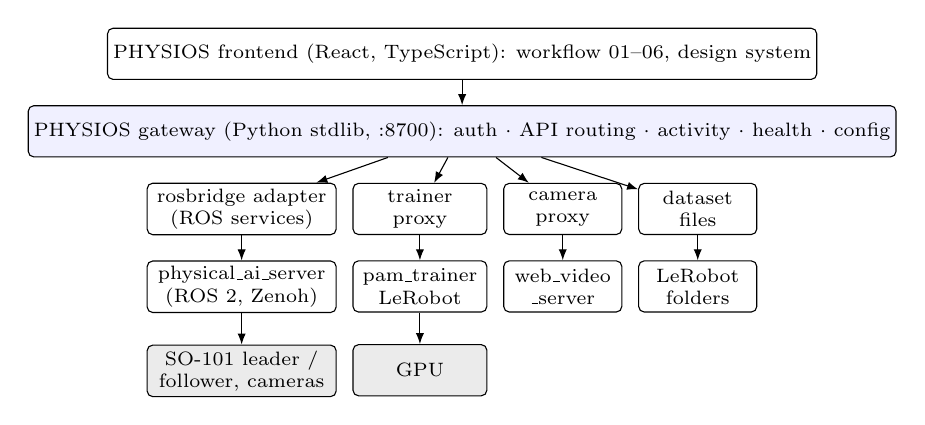
\begin{tikzpicture}[font=\scriptsize, node distance=3.2mm and 2mm,
  box/.style={draw, rounded corners=2pt, align=center, minimum height=6.5mm, inner sep=2pt},
  layer/.style={draw, rounded corners=3pt, fill=black!4, inner sep=3pt}]
\node[box, minimum width=78mm] (fe) {PHYSIOS frontend (React, TypeScript): workflow 01--06, design system};
\node[box, minimum width=78mm, below=of fe, fill=blue!6] (gw) {PHYSIOS gateway (Python stdlib, :8700): auth $\cdot$ API routing $\cdot$ activity $\cdot$ health $\cdot$ config};
\node[box, below=of gw, xshift=-28mm, minimum width=24mm] (ros) {rosbridge adapter\\(ROS services)};
\node[box, right=of ros, minimum width=17mm] (tr) {trainer\\proxy};
\node[box, right=of tr, minimum width=15mm] (cam) {camera\\proxy};
\node[box, right=of cam, minimum width=15mm] (ds) {dataset\\files};
\node[box, below=of ros, minimum width=24mm] (pas) {physical\_ai\_server\\(ROS 2, Zenoh)};
\node[box, below=of tr, minimum width=17mm] (pt) {pam\_trainer\\LeRobot};
\node[box, below=of cam, minimum width=15mm] (wvs) {web\_video\\\_server};
\node[box, below=of ds, minimum width=15mm] (lr) {LeRobot\\folders};
\node[box, below=4mm of pas, minimum width=24mm, fill=black!8] (arm) {SO-101 leader /\\follower, cameras};
\node[box, below=4mm of pt, minimum width=17mm, fill=black!8] (gpu) {GPU};
\foreach \a/\b in {fe/gw, gw/ros, gw/tr, gw/cam, gw/ds, ros/pas, tr/pt, cam/wvs, ds/lr, pas/arm, pt/gpu}
  \draw[-{Latex[length=1.4mm]}] (\a) -- (\b);
\end{tikzpicture}}
\caption{PHYSIOS layers. Only the two top layers are new; everything below is reused
unchanged (R2).}
\label{fig:arch}
\end{figure}

\subsection{Gateway}
The gateway is a threaded HTTP server written against the Python standard library only, so it
runs in any Python~$\geq$3.9 without a virtual environment. Its parts are:
\begin{itemize}
\item a \textbf{rosbridge client} (RFC~6455 implementation) with reconnection, which exposes typed
operations (robot types, cameras, policies, task commands, planning and data commands) and
translates failures into structured errors such as \texttt{ros\_service\_missing} with a remedy
(e.g.\ ``start the Zenoh router first'');
\item a \textbf{training proxy} that forwards \texttt{/api/v1/trainer/*} unchanged, preserving the
training service's own same-origin and confirmation-token checks;
\item a \textbf{camera proxy} for MJPEG streams, so the browser uses one origin;
\item \textbf{read-only dataset access} with HTTP Range support for episode videos and a streamed
\texttt{.tar.gz} export;
\item \textbf{health and host metrics}: six live checks (gateway, trainer, rosbridge, ROS node,
camera, datasets), CPU utilisation from \texttt{/proc/stat} deltas, and host information from
the training service's environment module (imported, not copied);
\item an \textbf{activity log} persisted as JSON lines; and
\item optional \textbf{authentication} (Section~\ref{sec:auth}).
\end{itemize}
The gateway is about 1.6\,k lines of Python.

\subsection{Frontend}
The frontend is a Vite-built React~18 application in strict TypeScript (about 5.8\,k lines),
with no router, state-management, chart or component library; three.js is loaded only for the
robot viewer. Logic that is safety-relevant was ported from the earlier interface as code, not
as UI: the URDF loader and the one-joint hardware-test sequencer, which has its own unit tests
against a simulated servo.

\subsection{Deployment}
Two equivalent paths exist. Scripts start the gateway (and the training service if it is not
running), check every dependency and print service health; they never start motion. A
container image holds only the gateway and the built frontend, runs as an unprivileged user with
host networking next to the existing robot containers, mounts the repository and dataset cache
read-only, and declares a health check. The training service stays on the host because it
needs the operator's LeRobot environment and GPU.

\subsection{Authentication}\label{sec:auth}
On a loopback-only gateway the operating-system account is the security boundary. Setting an
operator token enables sign-in: tokens are compared in constant time; sessions are random
256-bit identifiers in HttpOnly, SameSite=Strict cookies with a configurable lifetime; scripts
may use a Bearer token; five failed attempts per address and minute trigger a one-minute block.
The gateway refuses to listen on a non-loopback address without a token. Cross-origin POST
requests and WebSocket upgrades are rejected regardless.

\section{Workflow Modules}\label{sec:workflow}
\textbf{Planning} uses the existing planning engine to generate per-episode placements of
objects and targets within a reachable workspace, validate them and version the approved
plan. \textbf{Recording} binds each take to a planned episode: the plan's instruction and set-up
are shown, the take is started through \texttt{/task/command}, and an optional review step
accepts or rejects the episode. \textbf{Data} lists datasets with review state, plays episode
videos, and supports validation, publishing and export.

\textbf{Training and optimisation.} Training commands are built from the installed
\texttt{lerobot-train --help}, shown verbatim and started only with a server-issued token that
matches the reviewed command. Logged metrics feed detectors for non-finite or exploding loss,
gradient explosion, stagnation, over-fitting (validation loss rising while training loss falls),
excessive clipping, memory pressure and data-loading bottlenecks. For a problem with onset
step $s$, an optimisation session restarts from the latest usable checkpoint before $s$ with
weights only (no optimiser state), running a \emph{control} with unchanged settings and up to
three trials, each changing levers that the policy actually supports. A trial with final metric
$m_t$ is recommended over the control $m_c$ only if
\begin{equation}
g = \frac{m_c - m_t}{|m_c|}\times 100\,\% \;\geq\; g_{\min},\qquad g_{\min}=5\,\%,
\end{equation}
otherwise the advice is to keep the original settings. Budgets bound the number of trials, GPU
time and per-trial duration.

\textbf{Evaluation} records robot trials per checkpoint. With $k$ successes out of $n$ trials,
the success rate is reported with the Wilson score interval
\begin{equation}
\frac{\hat p + \frac{z^2}{2n} \pm z\sqrt{\frac{\hat p(1-\hat p)}{n} + \frac{z^2}{4n^2}}}{1+\frac{z^2}{n}},\quad \hat p = \tfrac{k}{n},\; z = 1.96,
\end{equation}
which stays informative for the small $n$ typical of physical trials. Training metrics and
robot results are kept separate, and a recommendation is labelled robot-based only with at
least three evaluated trials.

\textbf{Inference} offers a dry-run model check (live inputs, safety-filtered outputs, nothing
published), a host rollout of models trained on the PC, and container inference of policies
stored on the robot side. \textbf{Robots} registers custom arms from URDF/Xacro archives with a
restricted Xacro expander that never executes code, validates the model, renders it, and
advances through four readiness stages (registered, ROS verified, hardware verified, data and
training ready).

\section{Safety Model}\label{sec:safety}
Motion can originate only from four operator actions: starting a recording take (the follower
then mirrors the leader arm), \emph{Run} in host rollout, \emph{Start} in container inference,
and \emph{Start motion} in the one-joint hardware test. The safeguards are layered:
\begin{enumerate}
\item \emph{Start-up.} Neither the scripts nor the container start recording, inference or a
rollout.
\item \emph{Typed confirmation.} Run and Start require a checklist and typing ``run''. The gateway
independently rejects inference commands without \texttt{confirm: true} (HTTP 428), so a script
or a modified page cannot bypass the dialog.
\item \emph{Two-step host rollout.} \emph{Load} starts the worker with the arm still; only
\emph{Run} publishes commands.
\item \emph{Worker-side limits.} Each command is clipped to a joint envelope derived from the
demonstrations (+5\,\%, tightenable, widenable by at most 10\,\%), a per-step change limit and
a lead limit; stale camera or joint data ($>0.5$\,s) or a missing operator heartbeat ($>2$\,s)
cause the arm to hold; a maximum duration and an emergency stop end the run; the worker refuses
to start if another node publishes on the command topic.
\item \emph{Custom robots.} The hardware test uses a single-use, server-issued plan (at most
0.1\,rad at 0.2\,rad/s towards mid-range, valid 180\,s); a pre-hold detects inverted joints or
offsets before the intended motion; the server judges the recorded samples. Changing mappings or
limits withdraws the corresponding readiness stages.
\end{enumerate}
A software stop is not an emergency stop; the procedure requires a hardware stop within reach.

\section{Interface Design}\label{sec:ui}
The interface keeps the visual language operators already knew from the earlier tool---soft
grey canvas, white sheets, black active capsules, numbered workflow rail---so that adoption
does not require retraining. Version 1.1 optimises it for information density: hairline-bordered
cards with 14\,px radius, a 78\,px rail, compact controls and tables, and work areas up to
1760\,px wide. Recording and inference use a \emph{console} layout (Fig.~\ref{fig:record}):
robot type and connection state top left, live cameras centre, the planned episode with its
instruction and set-up on the right, and a control bar with Start/Stop/Retry/Next/Finish, phase,
progress and host resources at the bottom. Below 1100\,px the console stacks vertically; below
640\,px the rail becomes a bottom navigation bar. Every page shows a disconnected state with the
back end's own explanation instead of empty or invented data (R4).

\begin{figure*}[t]
\centering
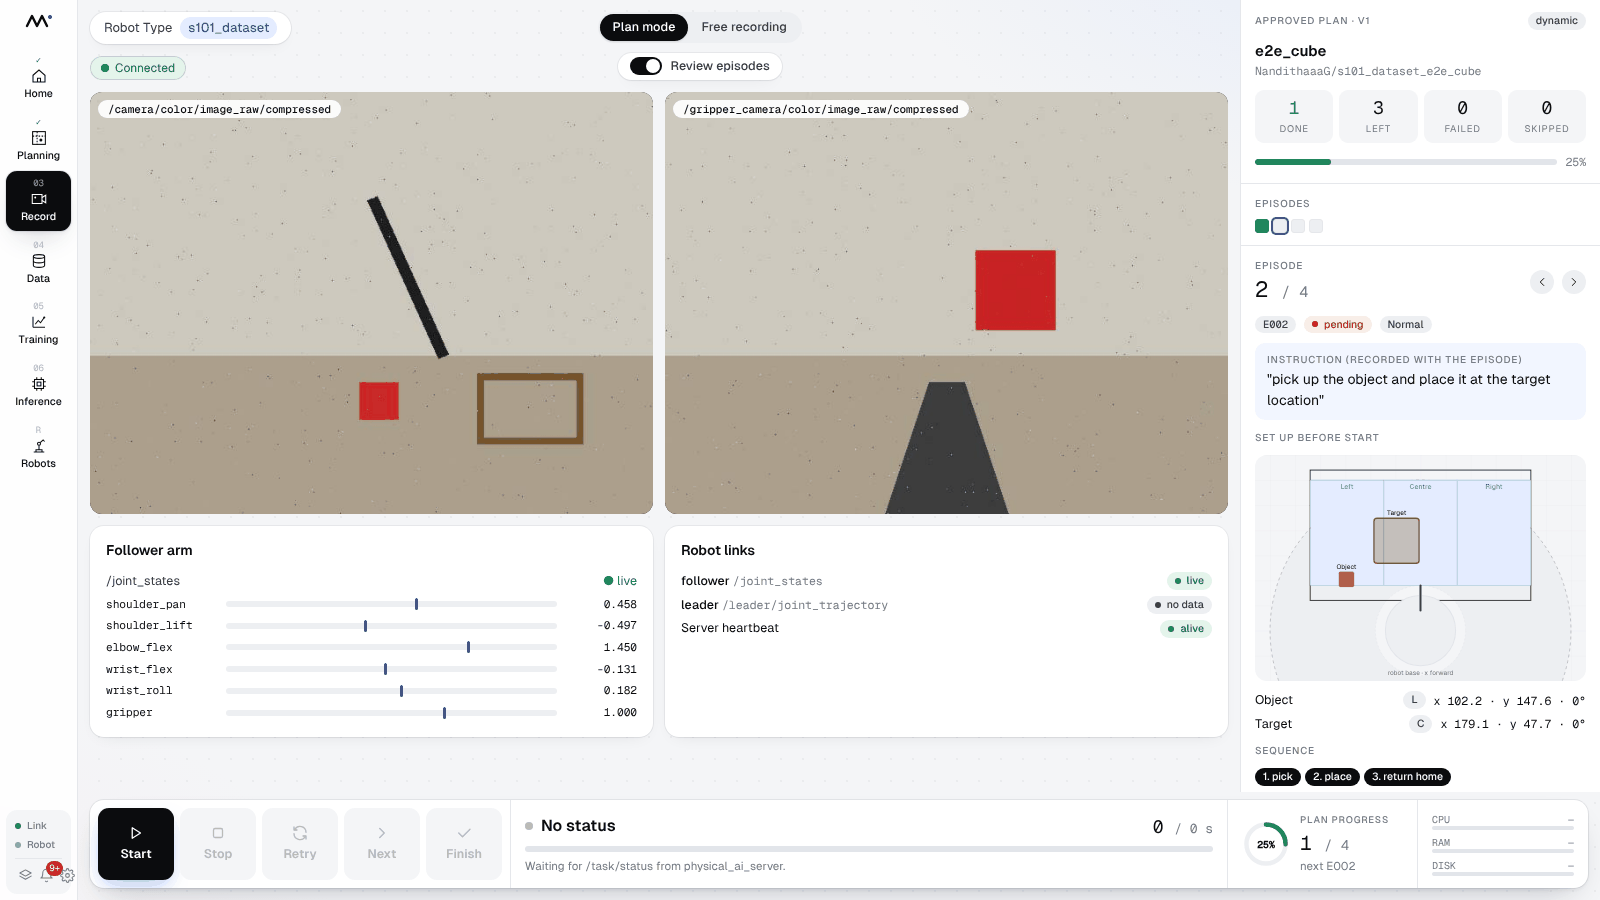
\includegraphics[width=0.82\textwidth]{03-record.png}
\caption{Record console in PHYSIOS 1.1 (simulated robot side): planned episode E002 with its
instruction and set-up, live cameras and joints, and the control bar.}
\label{fig:record}
\end{figure*}

\section{Validation}\label{sec:validation}
All tests were run in a sandbox without robot or GPU. The robot side was represented by the
\emph{real} planning-engine code behind a rosbridge stand-in with a simulated recorder; the
trainer was the \emph{real} training service with a stub \texttt{lerobot-train} that writes
logs and checkpoints and diverges for certain settings; custom-robot tests used a simulated
three-joint arm. Table~\ref{tab:tests} summarises the results on the final build.

\begin{table}[t]
\centering
\caption{Automated validation of PHYSIOS 1.1.0 (11 Nov 2026)}
\label{tab:tests}
\setlength{\tabcolsep}{3pt}
\begin{tabular}{@{}lr@{}}
\toprule
Suite & Result \\
\midrule
Gateway (API, adapters, sign-in) & 20 passed \\
Frontend units (hardware-test sequencer, helpers) & 8 passed \\
Type check and production build & clean \\
Browser walk-through, all modules & 14/14 steps \\
Sign-in walk-through (script / container) & 5/5, 5/5 \\
Training service (unchanged) & 91 passed, 1 skipped \\
Planning engine (unchanged) & 45 passed \\
Container: health check, six service checks & healthy, 6/6 \\
\bottomrule
\end{tabular}
\end{table}

The walk-through covers robot selection; plan creation, validation and activation; a
plan-mode take with review; dataset browsing, video playback and export; a token-confirmed
training run; diagnosis of a diverging run and a control trial; robot evaluation with a
confidence interval; inference compatibility and envelope; and the custom-robot path up to an
authorised one-joint test, in which 108 commands were published, none before Start, with all
other joints held. In the inference step, the dry-run load fails as expected because the
sandbox has no PyTorch; the interface shows the worker's log rather than a fabricated result.
The container was built on a substitute Ubuntu~24.04/Python~3.12 base because public registries
were unreachable from the sandbox.

\section{Limitations and Future Work}
The central limitation is that no result above was obtained on the physical SO-101 or with
GPU training. Outstanding checks are recording and camera streams through PHYSIOS, real
SmolVLA training and an optimisation session from a real checkpoint, a supervised low-speed
host rollout, and the hardware test on the real arm. Authentication uses a shared operator
token without per-user roles, and the gateway does not terminate TLS. Custom-robot server
configurations must still be installed by hand. Future work includes measuring how much the
planned-collection and review steps reduce the number of demonstrations needed for a reliable
grasp, camera-condition matching between training and deployment, and per-user audit trails.

\section{Conclusion}
PHYSIOS turns a set of capable but separate robot-learning tools into one independent
application with a single API, a dense and consistent operator interface, layered motion
safety and reproducible deployment, while leaving the robot-side software untouched. The
simulated validation is complete for all modules; physical validation on the SO-101 is the
next step.

\begin{thebibliography}{99}
\bibitem{rt2} A.~Brohan \emph{et al.}, ``RT-2: Vision-language-action models transfer web knowledge to robotic control,'' in \emph{Proc. Conf. Robot Learning (CoRL)}, 2023.
\bibitem{openvla} M.~J.~Kim \emph{et al.}, ``OpenVLA: An open-source vision-language-action model,'' in \emph{Proc. Conf. Robot Learning (CoRL)}, 2024.
\bibitem{pi0} K.~Black \emph{et al.}, ``$\pi_0$: A vision-language-action flow model for general robot control,'' arXiv:2410.24164, 2024.
\bibitem{smolvla} M.~Shukor \emph{et al.}, ``SmolVLA: A vision-language-action model for affordable and efficient robotics,'' arXiv:2506.01844, 2025.
\bibitem{act} T.~Z.~Zhao, V.~Kumar, S.~Levine, and C.~Finn, ``Learning fine-grained bimanual manipulation with low-cost hardware,'' in \emph{Proc. Robotics: Science and Systems (RSS)}, 2023.
\bibitem{diffusion} C.~Chi \emph{et al.}, ``Diffusion policy: Visuomotor policy learning via action diffusion,'' in \emph{Proc. Robotics: Science and Systems (RSS)}, 2023.
\bibitem{lerobot} R.~Cadene \emph{et al.}, ``LeRobot: State-of-the-art machine learning for real-world robotics in PyTorch,'' 2024. [Online]. Available: \url{https://github.com/huggingface/lerobot}
\bibitem{ros2} S.~Macenski, T.~Foote, B.~Gerkey, C.~Lalancette, and W.~Woodall, ``Robot Operating System 2: Design, architecture, and uses in the wild,'' \emph{Science Robotics}, vol.~7, no.~66, 2022.
\bibitem{pat} ROBOTIS, ``Physical AI Tools,'' 2025. [Online]. Available: \url{https://github.com/ROBOTIS-GIT/physical_ai_tools}
\bibitem{zenoh} Eclipse Foundation, ``Eclipse Zenoh.'' [Online]. Available: \url{https://zenoh.io}
\bibitem{rosbridge} C.~Crick, G.~Jay, S.~Osentoski, B.~Pitzer, and O.~C.~Jenkins, ``Rosbridge: ROS for non-ROS users,'' in \emph{Robotics Research}, Springer Tracts in Advanced Robotics, vol.~100, 2017, pp.~493--504.
\bibitem{rfc6455} I.~Fette and A.~Melnikov, ``The WebSocket protocol,'' IETF RFC 6455, 2011.
\end{thebibliography}

\end{document}
